% !TEX root =../thesis-letomes.tex

\chapter{Search Strategies}
\section{Evolution Strategies} \label{sec:ES}
OpenAI released a blog post \cite{Karpathy} with accompanying paper \cite{Salimans2017} in March 2017, where they announced ``Our finding continues the modern trend of achieving strong results with decades-old ideas''. Intuitively ES in a “guess and check” optimization process, where we start with some random parameters and then repeatedly 1) tweak the guess a bit randomly, and 2) move our guess slightly towards whatever tweaks worked better.

The team applied evolution strategies (ES) to two reinforcement learning (RL)\footnote{Reinforcement learning is an area of machine learning concerned with how software agents ought to take actions in an environment so as to maximize some notion of cumulative reward.} scenarios and compared the performance with typical deep RL problems:

\begin{enumerate}
    \item MuJoCo\footnote{MuJoCo stands for Multi-Joint dynamics with Contact, and is a ``physics engine aiming to facilitate research and development in robotics, biomechanics, graphics and animation, and other areas where fast and accurate simulation is needed''. See \url{http://www.mujoco.org}} (see \cref{fig:mujoco}) trained faster with ES than A3C\footnote{Asynchronous Advantage Actor Critic (A3C), published in 2016 \cite{Mnih2016}, is a class of deep RL algorithms that is still close to state of the art among deep RL algorithms.}.
    \item Atari game playing (see \cref{fig:atari}) trained to similar performance with ES in 1 hour compared to 1 day with A3C. Atari games have also become a popular problem space for deep RP researchers
\end{enumerate}

\begin{figure}[H]
    \centering
    \subfloat[MuJoCo: Creatures resembling a dog, 4-legged spider and worm learn to move forward. (Source: \cite{Karpathy})]{
        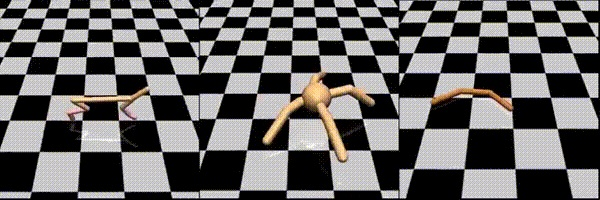
\includegraphics[width=0.46\linewidth]{fig/MuJoCo}
        \label{fig:mujoco}
    }
    \hfill
    \subfloat[Atari games are popular to RL algorithm research. Here: Brekaout (left) and Space Invaders (right) (Source: \cite{Deshpande}).]{
        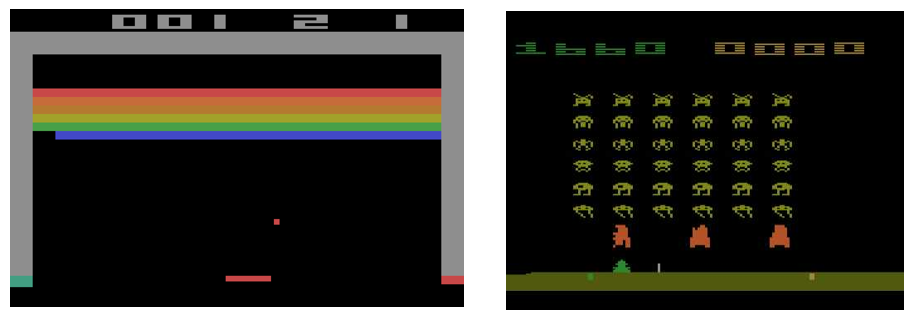
\includegraphics[width=0.46\linewidth]{fig/Atari}
        \label{fig:atari}
    }
    \caption{Two Applications used for testing RL algorithms: MuJoCo and Atari.}
    \label{fig:rl}
\end{figure} 

To achieve the signal needed for learning, i.e. exploration, noise must be somehow injected into the system:
- For RL, noise is injected into the agent's \emph{actions}.
- For ES, noise is injected directly into the \emph{parameters}.

We are basing our machine learning efforts on the Evolution Strategy (ES) algorithm outlined by Salimans et al. \cite{Salimans2017} using ES--it being a gradient estimator--makes sense in optimization scenarios where calculating an exact gradient is expensive, or even impossible. The idea is to sample around a starting point, and use a weighted average fitness score to pick a direction to move each cycle. It is generally applicable to unsupervised problems, such as ours; a reinforcement learning problem. There are several flavors of the concept under the ES umbrella term: Covariance Matrix Adaptation (CMA-ES), Natural Evolution Strategy (NES), and Exponential NES, to name a few. The one used in \cite{Salimans2017} and by extension in our project is NES. Its exact implementation details will follow:

\subsection{Theoretical Advantages and Disadvantages of ES Compared to RL}
The advantages of ES is outlined in \cite{Karpathy} and can be summarized as follows:
\begin{enumerate}
    \item No need for back propagation.
    \begin{itemize}
        \item Makes code shorter and 2-3x faster
        \item Memory saving: not necessary to keep episode recordings for later update.
        \item No need to worry about exploding gradients in recurrent neural networks.
        \item We can explore larger classes of policy functions, including networks that are not differentiable.

    \end{itemize}
    \item Highly parallelizable.
    \begin{itemize}
        \item ES workers communicate scalars, RL workers communicate entire parameter vectors -> easy to obtain linear speedups with more CPU cores.
    \end{itemize}
    \item Higher robustness.
    \begin{itemize}
        \item Has fewer hyperparameters. Several hyperparameters that are difficult to set in RL implementations are side-stepped in ES. The details are a little technical / not elaborated in blog post.
    \end{itemize}

    \item Structured exploration.
    \begin{itemize}
        \item Due to the noise being injected in parameter space, not actions, ES can use deterministic policies and achieve consistent exploration (instead of "jittering on the spot"). 
    \end{itemize}
    \item Credit assignment over long time scales
    \begin{itemize}
        \item By studying both ES and RL gradient estimators mathematically we can see that \emph{ES is an attractive choice especially when the number of time steps in an episode is long, where actions have long-lasting effects}, or if no good value function estimates are available.
    \end{itemize}
\end{enumerate}

\subsubsection{ES Challanges}

A core problem in ES is that adding noise in parameters must lead to different outcomes to obtain some gradient signal. It turns out that virtual batch normalization can help alleviate this problem \cite{Karpathy}.

Another problem is that it doesn't really work on \emph{supervised learning}, i.e. in settings where we know the/a solution/truth and want to use that to train a neural network. Supervised learning problems include image classification, speech recognition, or most other tasks in the industry, where one can compute the exact gradient of the loss function with backpropagation. For example, in the preliminary experiments it was found that using ES to estimate the gradient on the MNIST digit recognition task can be as much as 1,000 times slower than using backpropagation\cite{Karpathy}.

Therefore, \emph{it is only in RL settings, where one has to estimate the gradient of the expected reward by sampling, where ES becomes competitive}.

\subsubsection{ES Advantages Summary}
In conclusion we are interested in ES as an optimization algorithm for LETO search mainly because it has advantages in:
\begin{itemize}
    \item Reduced code complexity
    \item Ease of scaling (to large-scale distributed settings)
    \item It does not suffer in settings with sparse rewards, such as is the case in searching for LETOs.
\end{itemize}

\subsection{NES Algorithm}
In formal terms: \emph{``Let F denote the objective function acting on parameters θ. NES algorithms represent the population with a distribution over parameters \(p_\psi (\theta)\)—itself parameterized by $\psi$—and proceed to maximize the average objective value \(E_{\theta \sim p_\psi}\) over the population by searching for $\psi$ with stochastic gradient ascent. Specifically, using the score function estimator for $\nabla_\psi E_{\theta \sim p_\psi} F(\theta)$, [...] NES algorithms take gradient steps on $\psi$ with the following estimator:''} \cite[p.~2]{Salimans2017}
\begin{equation}
    \nabla_\psi E_{\theta \sim p_\psi} F(\theta)
    = E_{\theta \sim p_\psi} \{F(\theta)~\nabla_\psi~log~p_\psi(\theta)\}
\end{equation}
In our problem, \(F\) is the score returned by our environment (the Earth-Moon or Earth-Mars-Sun system)(required $\Delta v$ for our spacecraft's path) with \(\theta\) representing a single path in the environment and \(\psi\) being the parametrization of that path (example launch parameters: starting position of spacecraft, angle of burn vector at time of maneuver, and magnitude of that burn vector). The algorithm mutates the launch parameters \(\psi\), checks how the resulting path \(\theta\) performs in the environment \(F\) and moves around the resulting n-dimensional optimization space with gradient descent along its estimated gradient, defined by a normally distributed weighted point cloud \(\epsilon\).

\begin{figure}
    \centering
    \subfloat[Starting at some random point, the first iteration computes the fitness of a surrounding point cloud ($\epsilon$), and takes a step of size $\alpha$ in the direction of the weighted mean of $\epsilon$.]{
        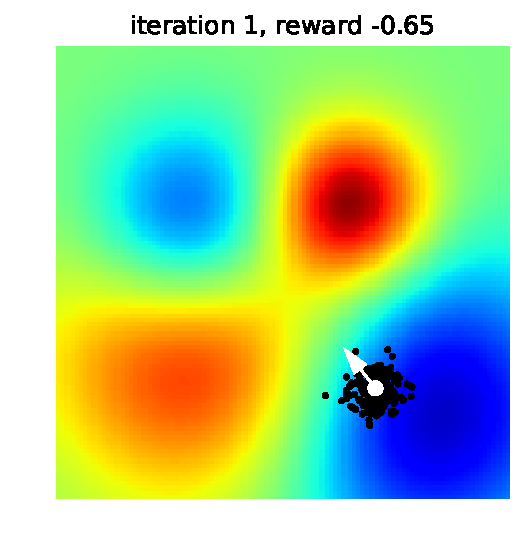
\includegraphics[width=0.46\linewidth]{fig/ES_basic_0}
        \label{fig:esbasic0}
    }
    \hfill
    \subfloat[this process continues each iteration, until we find ourselves at a local maximum (this example version is doing gradient \textit{ascent})]{
        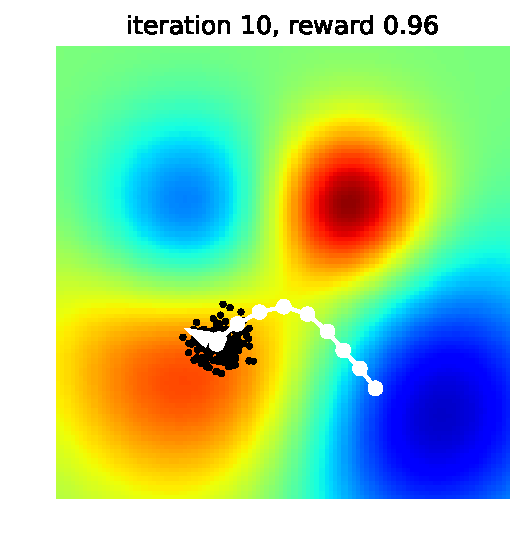
\includegraphics[width=0.46\linewidth]{fig/ES_basic_9}
        \label{fig:esbasic9}
    }
    \caption{the fundamental ES algorithm illustrated in a toy problem. Generated from code based on \cite{Salimans2017}}
    \label{fig:esbasic}

\end{figure}

In genetic algorithm terms, the input parameters $\psi$ are the genotype, the resultant path $\theta_\psi$ is the phenotype, and the fitness is of course  $F(\theta_\psi)$. \cite{Tomassini2005}. Since we simply input $\psi$ to the simulator that delivers $F(\theta_\psi)$, and $\theta$ is not really within the purview of the ES module, we will generally skip $\theta_\psi$, and simply write $F(\psi)$ instead, unless the distinction between geno- and phenotype is relevant. This also reflects the reality more precisely, with regards to our code.
\subsection{Modifications}
There are a number of modifications to the core ES idea of gradient descent with an estimated gradient, that are required for the algorithm to actually work in anything but the most ideal context. 

\subsubsection{Fitness Shaping}
Fitness shaping refers to the transformations one can perform on the output of $F$, generally in order to smoothen the optimization algorithm's movement. One such transformation that was particularly critical for our problem was rank transformation, i.e. for each gradient estimation distribution $F(\psi_t + \sigma\epsilon_i)$, we replace the value of $F_i$ with its index in the sorted list of $F_{0..n}$. This shaping is to prevent outliers from overly influencing the gradient estimate. If a value is extreme in one way or the other, it would otherwise either pull or push the next iteration $\psi_{t+1}$ proportionately. With rank transformation, this sensitivity to the random sampling of $\sigma\epsilon$ largely disappears. \cite{Wierstra2011}. 

Another fitness shaping approach that we tried was sub-par sample flattening. Since we are more interested in being pulled \textit{towards} good solutions than being pushed away from bad ones, we ignore the half of the estimation distribution $\sigma\epsilon$ that performs worse than the mean. We tried this both in and out of conjunction with rank transformation, but it did not perform particularly in either case, having a negligible influence.

\subsubsection{Antithetical Sampling}
Another measure to reduce the impact of variance in the sampling of $\sigma\epsilon$ is antithetical sampling. This means that for every point $\psi_t + \sigma\epsilon_i$ we sample, we evaluate its complement, $\psi_t - \sigma\epsilon_i$ as well. \cite{Salimans2017}. This means that there are always an equal number of points on either side of the distribution, and the estimated gradient is not thrown off by extreme stochastic outcomes in this regard.


\section{Fan Search}
In \cite{Saxe2015}, the search strategy was significantly simpler than here, and it serves as the point of comparison for our search efforts. The way it was done is that the same three parameters contained in $\psi$ were tested in a three-dimensional fan arrangement. For example, the starting position $\psi_{pos}$ was defined from 0 to $2\pi$, the burn angle $\psi_{ang}$ was defined between 0 and $-\frac{\pi}{4}$, and the burn vector's magnitude $\psi_{burn}$ was defined between 3 and 3.8. The search strategy was then to evaluate all superpositions of these three intervals, with e.g 100 values linearly spaced throughout each 'fan'. The set of values with the best score ($\psi\star$) would then be selected for refinement, where a smaller fan (tighter intervals) would be created, centered around $\psi\star$. The process would then repeat for some number of steps, constantly zeroing in on the best candidate.

For anyone with optimization experience it will be obvious that this method is very sensitive to local minimum issues. It doesn't multi-start, or compute any kind of gradient, definite or estimated. It relies heavily on empirically defined starting parameters for determining the initial search intervals, so it's very specific to this problem. It is, in short, not really universal, or particularly intelligent, and was thus seen as an obvious candidate for improvement in this project.

\section{Comparison of ES With Random Guessing Baseline}
In order to benchmark the performance of our ES implementation, we compared it with a baseline alternative; picking a random point within the problem space, and evaluating it, keeping it if it is the best we have seen. To find out which is best, there are two interesting metrics we can look at: 
\begin{itemize}
    \item Given a fixed budget of fitness evaluations, which algorithm finds the lowest value.
    \item Given some threshold value that is considered "good enough", which algorithm reaches that in the shortest time..
    \item ..or in the case where it is interesting to have multiple good candidate solutions, which algorithm outputs most of them in a given time.
\end{itemize}
Since the CPU-bound version of our algorithm takes several seconds to evaluate one fitness function, and the GPU version has had most of the pythonic\footnote{``Pythonic'' is a term often thrown around in the python programming community meaning ``doing things the way that is considered best practice in the Python'' that are in harmony with \href{https://www.python.org/dev/peps/pep-0020/}{The Zen of Python}, see \url{https://docs.python-guide.org/writing/style/}} convenience compromised, we pre-computed the fitness values in a promising cutout of the problem space. The 1024x1024 grid seen in \cref{fig:golf_course_s1024} took approximately 40 hours to compute on an HPC node, and with it, we were able to rapidly iterate our algorithm, both for the purpose of running it with multi-start to alleviate randomness, and to test the various potential accuracy and convergence-speed optimizations that have been applied in the literature.
\begin{figure}[ht]
    \centering
    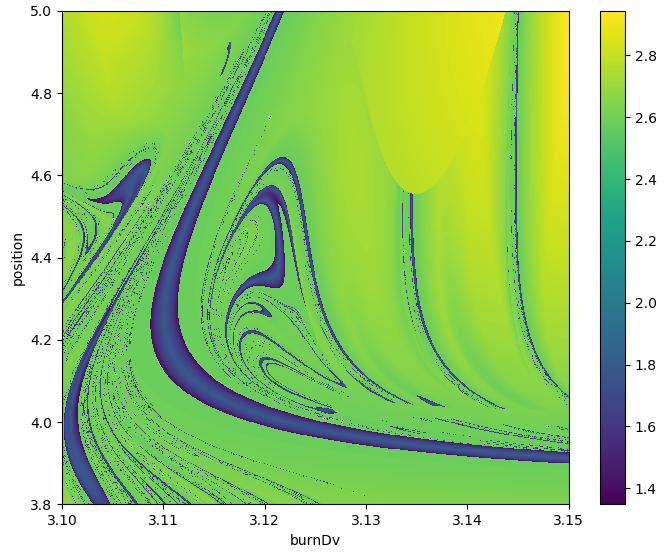
\includegraphics[width=\linewidth]{fig/golf_course_s1024.png}
    \caption{1024x1024 resolution fitness map of the flattened problem space. A certain fractal quality seems to be present, consistent with \cite{Topputo2014}}
    \label{fig:golf_course_s1024}
\end{figure}